\chapter{Materiais e Métodos}
% ---

% ---
\section{Microcontroladores e Microprocessadores}
% ---

Para uma melhor eficiência no processamento de dados, na década de 70
começaram a ser utilizados microprocessadores em computadores \cite{martins2005sistemas}. 

Os microprocessadores são componentes dedicados ao processamento de informações com
capacidade de cálculos matemáticos e endereçamento de memória externa \cite{chase2007sistemas}.

\subsection{ESP8266}

O ESP8266 é um circuito totalmente integrado, com interfaces de I\\O digitais e analógicas e, ainda, interface WiFi, com um processador de 32 bits, capaz de executar a 160 MHz.

Os módulos baseados no microcontrolador ESP8266 representam um grande avanço na relação de preço-recursos e podem ser um componente muito interessante para suluções IoT.\cite {de2017internet}

\begin{figure}[htbp]
		\centering
		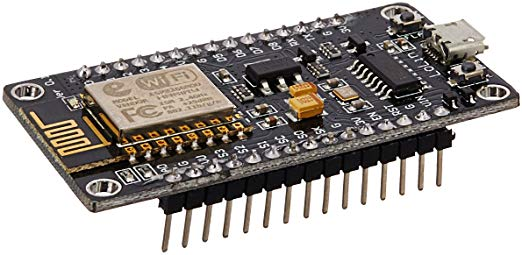
\includegraphics[scale=0.5]{figuras/esp8266_.jpg}
		\caption{ESP8266}
		\label{fig:09}
\end{figure}

\subsection{RaspberryPi}

Raspberry Pi é um minicomputador criado pela
Raspberry Pi Foundation com o objetivo de estimular o
ensino da ciência da computação nas escolas e
universidades. Apesar de o Raspberry Pi possuir o
hardware em uma única placa eletrônica de tamanho
reduzido, seu potencial de processamento é significativo.
O Raspberry Pi pode ser usado em diversos projetos
tecnológicos, como experimentos remotos nos quais sua
função é ser um Micro servidor web.\cite{crotti2013raspberrypi}

\begin{figure}[htbp]
		\centering
		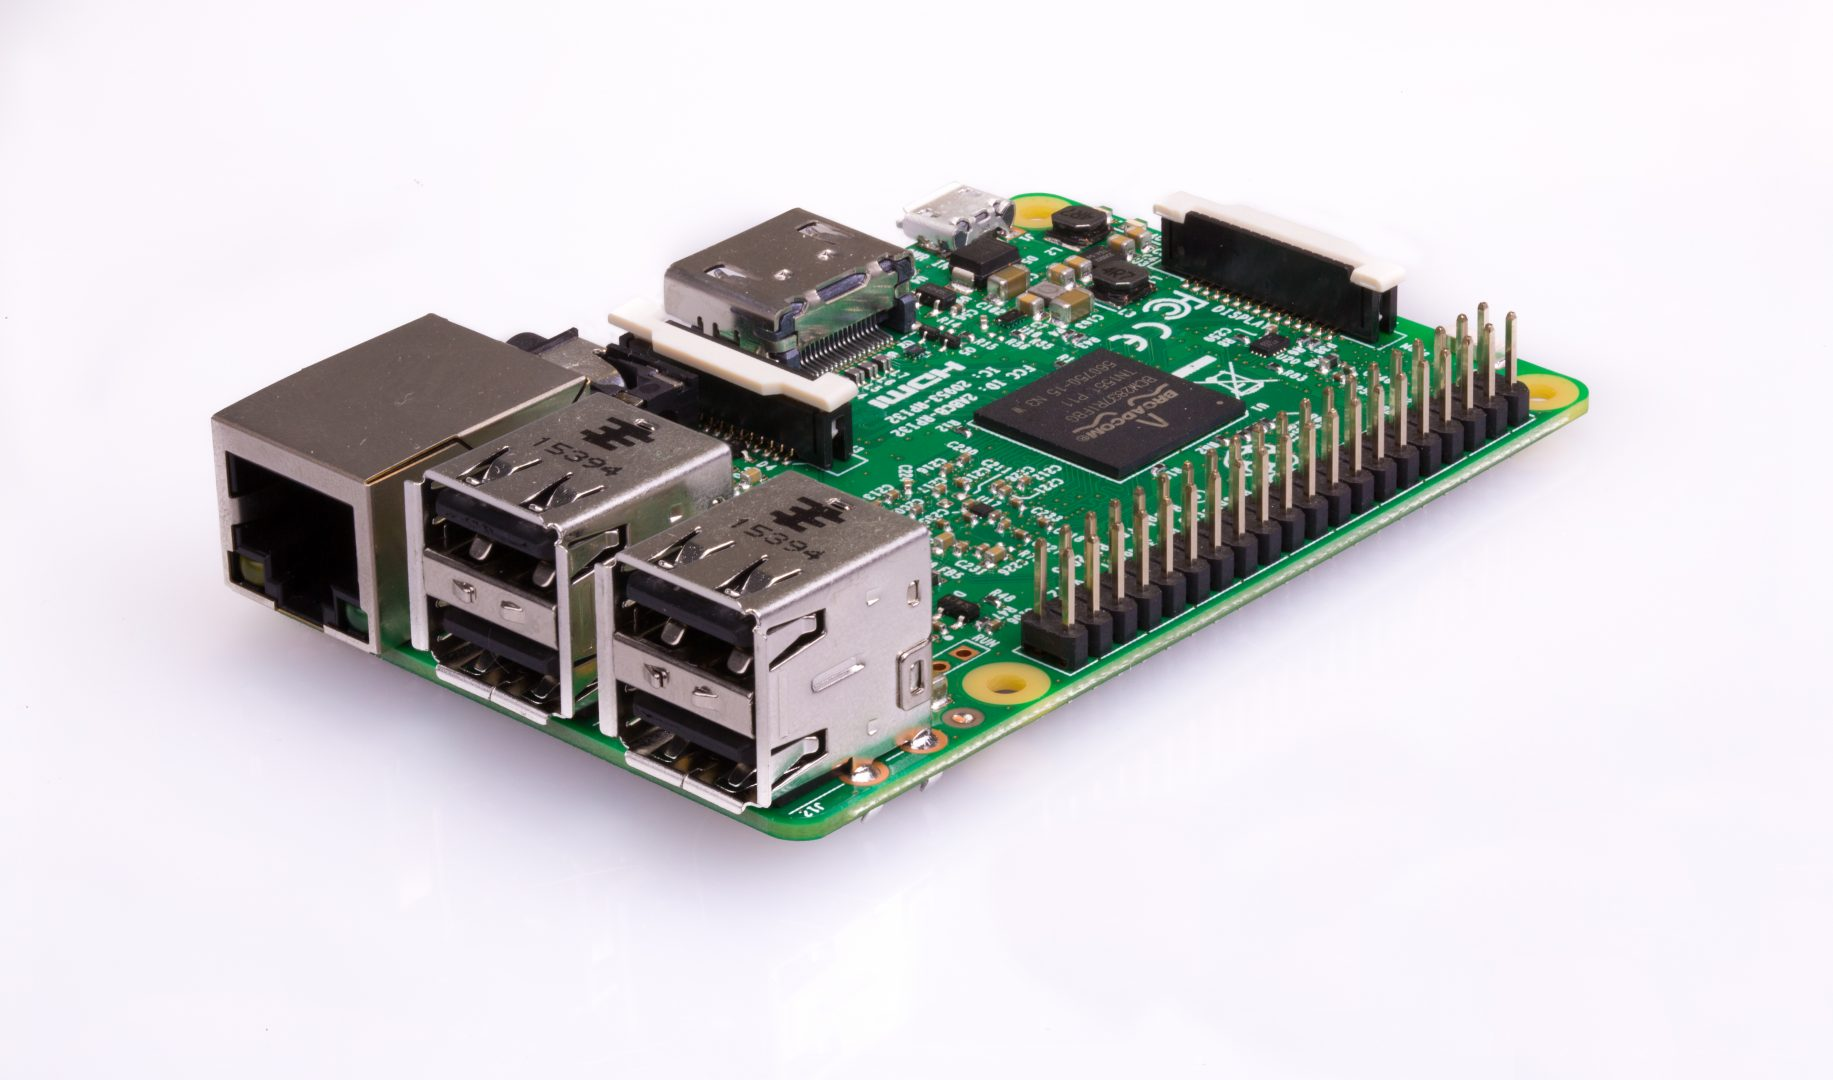
\includegraphics[scale=0.2]{figuras/raspberrypi.jpg}
		\caption{RaspberryPi}
		\label{fig:09}
\end{figure}

\section{Sensores e atuadores}

\subsection{Sensor de fluxo YF-S201}

São sensores do tipo turbina que medem a quantidade de líquido que passa pela tubulação, girando uma turbina que
gera pulsos de onda quadrada através de um sensor de efeito Hall\cite{roque2018sistema} O
sensor usa esse efeito para enviar um sinal PWM,e através desse pulso é possível mensurar a quantidade de água que passa pelo cata-vento no interior do sensor, cada pulso mede aproximadamente 2,25 mm.\cite{ms2017automaccao}

\begin{figure}[htbp]
		\centering
		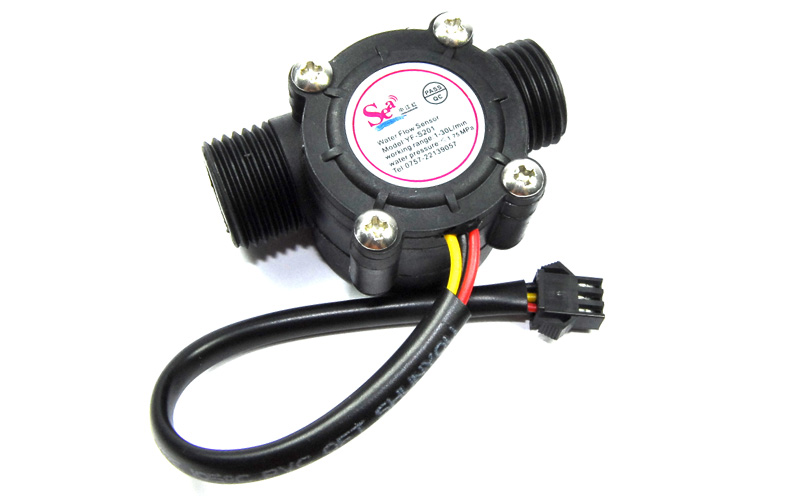
\includegraphics[scale=0.3]{figuras/yf-s201.jpg}
		\caption{Sensor de fluxo de água YF-S201}
		\label{sensor}
\end{figure}

\subsection{Teclado numérico}

\subsection{Relé de atuação}

\section{Softwares}

\subsection{MQTT Mosquitto}

\subsubsection{MQTT}

\subsection{Node.JS}

\subsubsection{Arquitetura de microsserviços}

\subsection{HomeAssistant}

\subsection{InfluxBD}

\subsection{Algum outro BD}